\begin{mainquestion}{capacitornetwork}{DC Capacitor Network}

Consider a network of eight capacitors arranged between two nodes A and B as shown below.

\begin{center}
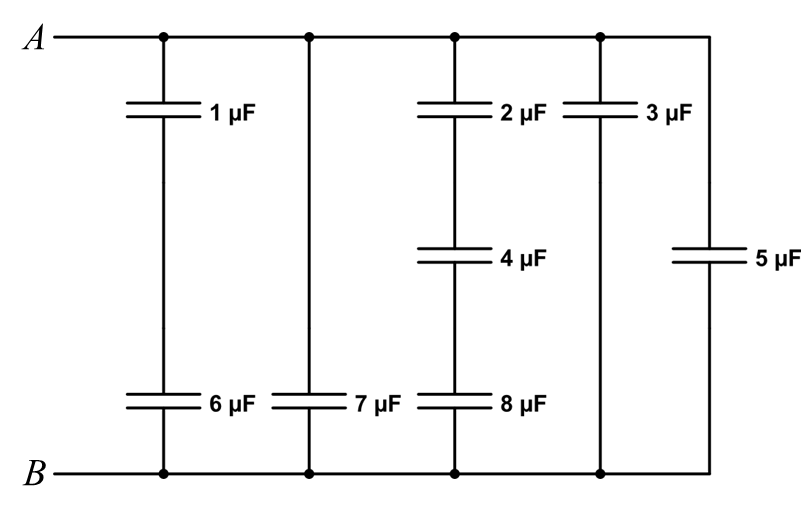
\includegraphics[width=0.8\textwidth]{questionbank/circuit_quantities/capacitor_network/v0/network_diagram.png}
\end{center}

% =========================================================
\begin{partquestion}{networksteadycurrent}
{Calculate the steady-state current through each capacitor if a 10~V battery is placed between A and B.}

\begin{answer}
At steady state, each capacitor will act like an open circuit and there will be no current through any of the capacitors. Therefore, all capacitor currents are zero.
\end{answer}
\end{partquestion}

% =========================================================
\begin{partquestion}{networksteadyvoltage}
{Calculate the voltage across each capacitor if a 10~V battery is placed between A and B.}

\begin{answer}
The voltage is a little more complicated. Each of the five parallel legs of the circuit have 10~V across them, so we can quickly assess that $V_{C7} = V_{C3} = V_{C5} = 10\text{ V}$.

For the first leg with two series capacitors, the total voltage across the capacitors is $V_{C1} + V_{C6} = 10\text{ V}$. We need one more equation relating the voltages between these two capacitors. The current through series capacitors must be the same, even as we approach steady state and the current becomes vanishingly small. The current is equivalent to the rate of change of charge, which implies that the total charge on each series capacitor must be the same. Since $Q_1 = Q_6$ we have:

\[
C_1 V_{C1} = C_6 V_{C6}
\]

Combining this with the previous result:

\begin{align*}
V_{C1} + \frac{C_1}{C_6}V_{C1} &= 10 \\
V_{C1} &= \frac{10C_6}{C_1 + C_6} \\
V_{C1} &= \frac{10\cdot6}{1 + 6} = \frac{60}{7}\text{ V} \\
\end{align*}

This gives $V_{C6} = 10 - \frac{60}{7} = \frac{10}{7}\text{ V}$.

For the leg containing three series capacitors, we have $Q_2 = Q_4 = Q_8$ and thus:

\[
C_2 V_{C2} = C_4 V_{C4} = C_8 V_{C8}
\]

With $V_{C2} + V_{C4} + V_{C8} = 10\text{ V}$:

\[
V_{C2} = \frac{10 C_4 C_8}{C_2 C_4 + C_2 C_8 + C_4 C_8} = \frac{10(4)(8)}{(2)(4) + (2)(8) + (4)(8)} = \frac{320}{56} = \frac{40}{7}\text{ V}
\]

We can then find:

\begin{align*}
V_{C8} &= \frac{C_2}{C_8}V_{C2} \\
&= \frac{2}{8}\cdot\frac{40}{7} = \frac{10}{7}\text{ V}
\end{align*}

and

\begin{align*}
V_{C4} &= \frac{C_2}{C_4}V_{C2} \\
&= \frac{2}{4}\cdot\frac{40}{7} = \frac{20}{7}\text{ V}
\end{align*}

\textbf{Summary of capacitor voltages:}
\begin{itemize}
  \item $V_{C1} = \frac{60}{7}\text{ V} \approx 8.57\text{ V}$
  \item $V_{C6} = \frac{10}{7}\text{ V} \approx 1.43\text{ V}$
  \item $V_{C3} = 10\text{ V}$
  \item $V_{C5} = 10\text{ V}$
  \item $V_{C7} = 10\text{ V}$
  \item $V_{C2} = \frac{40}{7}\text{ V} \approx 5.71\text{ V}$ 
  \item $V_{C4} = \frac{20}{7}\text{ V} \approx 2.86\text{ V}$
  \item $V_{C8} = \frac{10}{7}\text{ V} \approx 1.43\text{ V}$
\end{itemize}

\end{answer}
\end{partquestion}

\end{mainquestion}
